\documentclass{article}\usepackage[]{graphicx}\usepackage[]{color}
%% maxwidth is the original width if it is less than linewidth
%% otherwise use linewidth (to make sure the graphics do not exceed the margin)
\makeatletter
\def\maxwidth{ %
  \ifdim\Gin@nat@width>\linewidth
    \linewidth
  \else
    \Gin@nat@width
  \fi
}
\makeatother

\definecolor{fgcolor}{rgb}{0.345, 0.345, 0.345}
\newcommand{\hlnum}[1]{\textcolor[rgb]{0.686,0.059,0.569}{#1}}%
\newcommand{\hlstr}[1]{\textcolor[rgb]{0.192,0.494,0.8}{#1}}%
\newcommand{\hlcom}[1]{\textcolor[rgb]{0.678,0.584,0.686}{\textit{#1}}}%
\newcommand{\hlopt}[1]{\textcolor[rgb]{0,0,0}{#1}}%
\newcommand{\hlstd}[1]{\textcolor[rgb]{0.345,0.345,0.345}{#1}}%
\newcommand{\hlkwa}[1]{\textcolor[rgb]{0.161,0.373,0.58}{\textbf{#1}}}%
\newcommand{\hlkwb}[1]{\textcolor[rgb]{0.69,0.353,0.396}{#1}}%
\newcommand{\hlkwc}[1]{\textcolor[rgb]{0.333,0.667,0.333}{#1}}%
\newcommand{\hlkwd}[1]{\textcolor[rgb]{0.737,0.353,0.396}{\textbf{#1}}}%

\usepackage{framed}
\makeatletter
\newenvironment{kframe}{%
 \def\at@end@of@kframe{}%
 \ifinner\ifhmode%
  \def\at@end@of@kframe{\end{minipage}}%
  \begin{minipage}{\columnwidth}%
 \fi\fi%
 \def\FrameCommand##1{\hskip\@totalleftmargin \hskip-\fboxsep
 \colorbox{shadecolor}{##1}\hskip-\fboxsep
     % There is no \\@totalrightmargin, so:
     \hskip-\linewidth \hskip-\@totalleftmargin \hskip\columnwidth}%
 \MakeFramed {\advance\hsize-\width
   \@totalleftmargin\z@ \linewidth\hsize
   \@setminipage}}%
 {\par\unskip\endMakeFramed%
 \at@end@of@kframe}
\makeatother

\definecolor{shadecolor}{rgb}{.97, .97, .97}
\definecolor{messagecolor}{rgb}{0, 0, 0}
\definecolor{warningcolor}{rgb}{1, 0, 1}
\definecolor{errorcolor}{rgb}{1, 0, 0}
\newenvironment{knitrout}{}{} % an empty environment to be redefined in TeX

\usepackage{alltt}

\usepackage{amsmath, amssymb}
\usepackage{graphicx}
\usepackage{hyperref}
\IfFileExists{upquote.sty}{\usepackage{upquote}}{}
\begin{document}

\title{Pol Sci 630:  Problem Set 10: 2SLS, Matching, Outlier, Heckman}

\author{Prepared by: Anh Le (\href{mailto:anh.le@duke.edu}{anh.le@duke.edu})}

\date{Due Date: Tue, Nov 3, 2015, 12 AM (Beginning of Lab)}

\maketitle

\section{2SLS}

\subsection{Load dataset CigarettesSW from package AER}

\subsection{Plot the following}

What can we say about the relationship between tax, price, and packs? Note: This is a good way to show the relationship between 3 variables with a 2D plot.

\begin{knitrout}
\definecolor{shadecolor}{rgb}{0.969, 0.969, 0.969}\color{fgcolor}
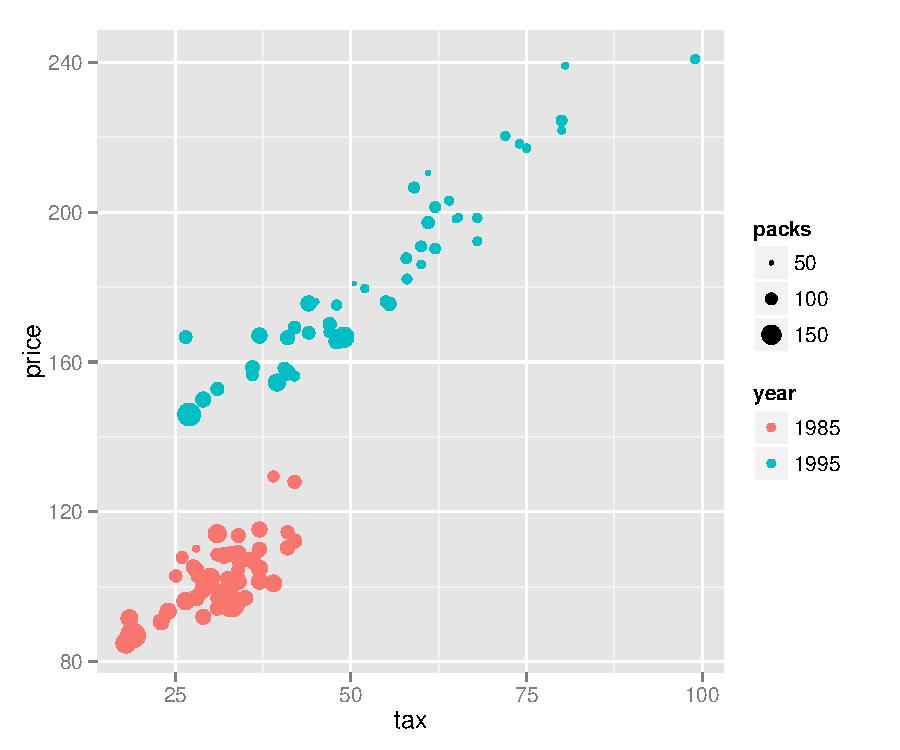
\includegraphics[width=\maxwidth]{figure/unnamed-chunk-1-1} 

\end{knitrout}

\subsection{Divide variable income by 1000 (for interpretability)}

\subsection{Run 2SLS}

Run 2SLS with \verb`ivreg`. Outcome: packs. Exogenous var: income. Endogenous var: price, whose instrument is tax. Interpret the coefficient of \verb`income` and \verb`price`.

\subsection{2SLS diagnostics: use F-test to check for weak instrument}

\subsection{2SLS by hand}

Run the 2SLS by hand, i.e. not using \verb`ivreg`, but run 2 stages of \verb`lm`. Do you get the same estimate from \verb`ivreg`?

\section{Matching}

\subsection{Load dataset lalonde from MatchIt, show covariate imbalance by plotting}

Plot the following. Hint: Look up \verb|position="dodge"| for ggplot2

\begin{knitrout}
\definecolor{shadecolor}{rgb}{0.969, 0.969, 0.969}\color{fgcolor}
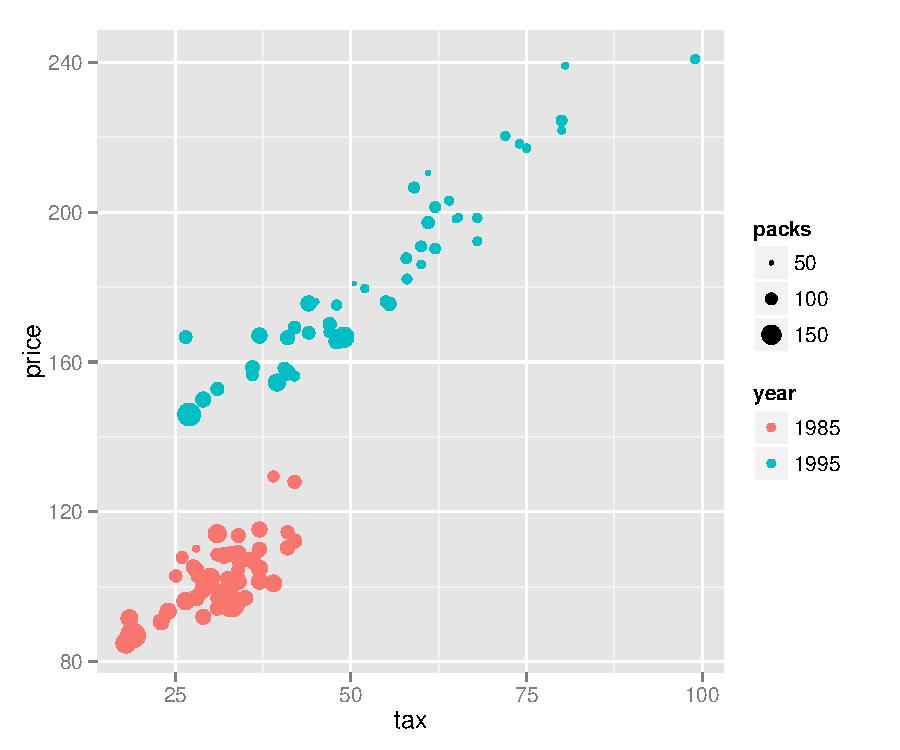
\includegraphics[width=\maxwidth]{figure/unnamed-chunk-2-1} 

\end{knitrout}

\subsection{See the effect of omitting an important variable}

Regress re78 against 1) treat, age, educ; 2) treat, age, educ, black. Do the treatment effect differ a lot? Why?

\subsection{Running CEM: Matching and check balance}

Match the treatment and the control group based on age, educ, and black. Check the balance

\subsection{Running CEM: Analysis after matching}

Run a weighted regression of re78 against 1) treat, age, educ, 2) treat, age, educ, and black. Do the treatment effect differ? Compare this result with part 2.

\section{Heckman}

\subsection{Load Mroz87 data from package sampleSelection}

\subsection{Run a Heckman model}

The selection variable is lfp. Run a heckman model with huswage, kid5, educ, city explaning the selection, and educ and city explaning the outcome variable log(wage). Interpret the result for the outcome model

\subsection{Outlier}

Load the anscombe dataset (the famous Anscombe quartet). Run a regression of y3 against x3, and find the outlier using any tools that we have discussed (DFbeta, cook distance, etc.)

Brownie point: Fit a linear model for y1 agains x1, y2 against x2, etc. What spooky thing did you notice?

\end{document}
